\documentclass{article}

\title{Assignment 3 : CS215}
\author{Akshat Chugh : 170050019 \\ Satvik Ambati : 170050101}

\usepackage{amsmath}
\usepackage{amssymb}
\usepackage{hyperref}
\usepackage{ulem}
\usepackage{graphicx}
\graphicspath{./}
\usepackage{enumerate}
\usepackage[margin=0.5in]{geometry}

\begin{document}
	\maketitle
\begin{enumerate}
\item
\begin{equation}
\hat{\mu}^{ML} = \frac{\sum_{i=1}^{n} x_i}{n}
\end{equation}
\begin{equation}
\hat{\mu}^{MAP1} = \frac{\bar{x} {\sigma_0}^2 + \frac{\mu_0 \sigma^2 } {n}}{{\sigma_0}^2 + \frac{\sigma^2} {n}}
\end{equation}
\begin{equation}
\hat{\mu}^{MAP2} = \frac{\sum_{i=1}^{n} x_i}{n}
\end{equation}
The maximum posterior estimate in case of a uniform prior is equal to the maximum likelihood estimate.
\\ \\ \\
\begin{center}
	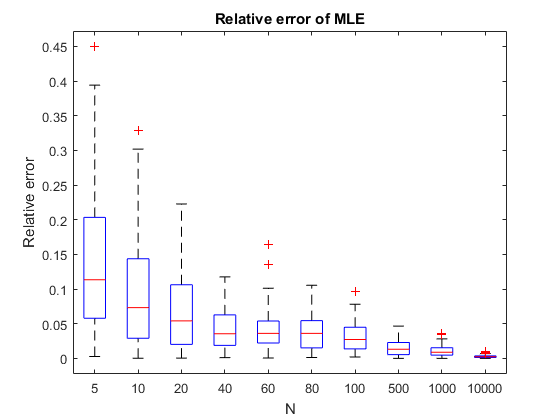
\includegraphics[scale=0.8]{p1_mle.png}
	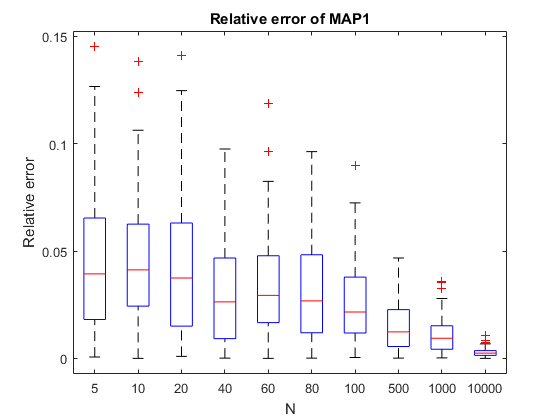
\includegraphics[scale=0.8]{p1_map1.png} 
	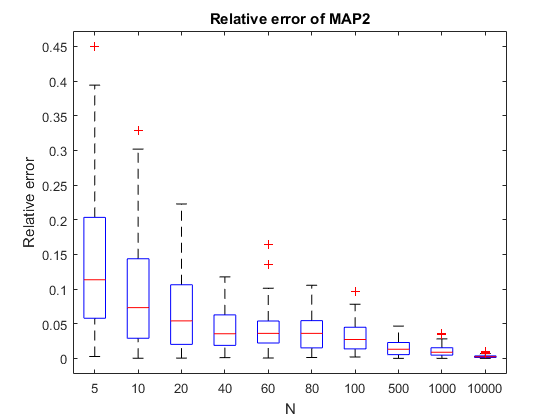
\includegraphics[scale=0.8]{p1_map2.png}
	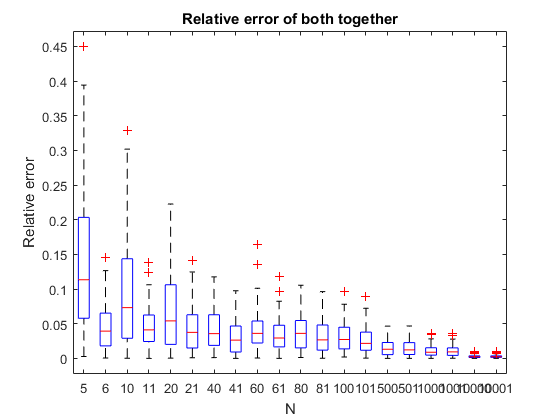
\includegraphics[scale=0.8]{p1_both.png}
\end{center} 

In the above graph, every alternate box starting with the first denotes the relative error plot of MLE
and the other set of alternate boxes starting with the second box denotes the relative error plot of Maximum Posterior estimate in case of Gaussian Prior. MAP2 is the same as MLE. 


For very large values of $n$, the relative error for all the three estimates i.e. MLE, MAP1 and MAP2 is very small. \\
The relative error for MLE and MAP2 is spread across a wider range than the relative error for MAP1.
\begin{enumerate}[(i)]
\item The relative error in case of both MLE and MAP2 decreases with increase in $N$. 
\\ The relative error in case of MAP1, initially decreases or almost remains the same or increases slightly with increase in $n$ (for smaller values of $n$); but at higher values of $n$ it decreases with increases in $n$. 
\item For smaller values of $n$, the relative error for MLE and MAP2 is greater than the relative error for MAP1. \\ 
Since with the increase in $n$, MAP1 tends to the Maximum Likelihood estimate(MLE), the relative error for MAP1 tends to the relative error for MLE and MAP2. \\
Therefore, MAP1 (Maximum posterior estimate with the given Gaussian prior) is the best estimate, as the relative error is almost the least for all values of $n$ among the given three estimates. 
\end{enumerate}

\end{enumerate}
\end{document}